\section{Stacionární poruchová metoda}
\label{sec:PoruchovaMetoda}
\begin{theory}   
    Mějme Hamiltonián $\operator{H}$, který lze rozložit na součet
    \begin{equation}
        \operator{H}=\operator{H}_{0}+\lambda\operator{H}_{\ti{I}}
    \end{equation}
    tak, že spektrum $\operator{H}_{0}$ je známé a {\bf nedegenerované},
    \begin{subequations}
        \begin{align}
            \operator{H}_{0}\ket{\phi_{m}}&=E_{m}^{\hi{0}}\ket{\phi_{m}},\\
            \braket{\phi_{m}}{\phi_{n}}&=\delta_{mn},\\
            \sum_{m}\ket{\phi_{m}}\bra{\phi_{m}}&=\operator{1},
        \end{align}
    \end{subequations}
    a $\operator{H}_{\ti{I}}$ je malá porucha (interakce) řízená parametrem $\lambda$ 
    ($\lambda=0$ v neporušeném případě, řešení pro $\lambda=1$ hledáme; mocnina $\lambda$ ve výsledku koresponduje s řádem opravy).

    Předpokládáme, že vlastní vektor Hamiltoniánu $\operator{H}$ a příslušné vlastní energie lze vyjádřit ve tvaru součtu
    \begin{subequations}
        \begin{align}
            \ket{\chi_{m}(\lambda)}&=\sum_{n=0}^{\infty}\lambda^{n}\ket{\chi_{m}^{\hi{n}}},\\
            E_{m}(\lambda)&=\sum_{n=0}^{\infty}\lambda^{n}E_{m}^{\hi{n}},\\
            \operator{H}\ket{\chi_{m}(\lambda)}&=E_{m}(\lambda)\ket{\chi_{m}(\lambda)}
        \end{align}
    \end{subequations}
    přičemž platí $\ket{\chi_{m}^{\hi{0}}}\equiv\ket{\phi_{m}}$), kde $n$ udává řád opravy.
    Upustili jsme od normalizace vektorů $\ket{\chi_{m}^{\hi{n}}}$, avšak požadujeme, aby
    \begin{equation}
        \braket{\phi_{m}}{\chi_{m}(\lambda)}=1.
    \end{equation}
    V tomto označení platí pro první opravu 
    \begin{equation}
        \label{eq:Perturbation1}
        \important{
            \begin{aligned}
                E_{m}^{\hi{1}}&=\matrixelement{\phi_{m}}{\operator{H}_{\ti{I}}}{\phi_{m}}\\
                \ket{\chi_{m}^{\hi{1}}}&=\sum_{n\neq m}\frac{\matrixelement{\phi_{n}}{\operator{H}_{\ti{I}}}{\phi_{m}}}{E_{m}^{\hi{0}}-E_{n}^{\hi{0}}}\,\ket{\phi_{n}}
            \end{aligned}
        }
    \end{equation}
    a pro druhou opravu
    \begin{equation}
        \label{eq:Perturbation2}
        \important{
            E_{m}^{\hi{2}}=\sum_{n\neq m}\frac{\abss{\matrixelement{\phi_{n}}{\operator{H}_{\ti{I}}}{\phi_{m}}}}{E_{m}^{\hi{0}}-E_{n}^{\hi{0}}}\,.
        }
    \end{equation}
    Druhá oprava k základnímu stavu je vždy záporná.
    Výsledné stavy vyjádřené do daného řádu $N$ lze následně nanormovat.

    Pokud je spektrum $H_{0}$ {\bf degenerované}, pak uvedenou metodu nelze použít (to lze triviálně nahlédnout například z toho, že v prvním z výrazů v \eqref{eq:Perturbation1} by byla nejednoznačnost ve volbě vlastního vektoru $\ket{\phi_{m}}$, a také že ve jmenovatelích výrazů \eqref{eq:Perturbation1} a \eqref{eq:Perturbation2} bychom dostávali nuly).
    Předpokládejme, že platí
    \begin{subequations}
        \begin{align}
            \operator{H}_{0}\ket{\phi_{mj}}&=E_{m}\ket{\phi_{mj}},\\
            \braket{\phi_{mj}}{\phi_{mk}}&=\delta_{jk}\,.
        \end{align}
    \end{subequations}
    Všechny vlastní vektory v charakteristickém podprostoru operátoru $\operator{H}_{0}$ příslušejícím k vlastní hodnotě $E_{m}$ jsou indexovány druhým indexem. 
    První opravu $E_{mj}^{(1)}$ a příslušné vlastní vektory na tomto podprostoru získáme diagonalizací
    \begin{equation}
        \label{eq:PerturbationDegenerate}
        \important{
            \det\makematrix{
            \matrixelement{\phi_{m1}}{\operator{H}_{\ti{I}}}{\phi_{m1}} - E_{m}^{\hi{1}} & 
            \matrixelement{\phi_{m1}}{\operator{H}_{\ti{I}}}{\phi_{m2}} & \dotso \\
            \matrixelement{\phi_{m2}}{\operator{H}_{\ti{I}}}{\phi_{m1}} & 
            \matrixelement{\phi_{m2}}{\operator{H}_{\ti{I}}}{\phi_{m2}} - E_{m}^{\hi{1}} & \dotso \\
            \vdots & \vdots & \ddots
            }=0
        }.
    \end{equation}
    Porucha může degeneraci sejmout buď úplně, nebo jen částečně.
\end{theory}

\subsection{Porucha harmonického oscilátoru}
Částice hmotnosti $M$ se pohybuje v potenciálu jednorozměrného lineárního harmonického oscilátoru
\begin{equation}
    \operator{V}_{0}=\frac{1}{2}M\Omega^{2}\operator{x}^{2}
\end{equation}
s malou poruchou
\begin{equation}
    \operator{V}_{\mathrm{I}}=\lambda\cos\left(\kappa\operator{x}+\varphi\right)\,.
\end{equation}
\begin{enumerate}
\item
    Spočítejte 1. řád opravy energie základního stavu.
    
\item
    Vyjádřete střední hodnotu operátoru souřadnice $\operator{x}$ a střední hodnotu kvadrátu operátoru souřadnice $\operator{x}^{2}$ v tomto stavu.
\end{enumerate}

\begin{solution}
	\begin{enumerate}
	\item
		Oprava k energii je podle~\eqref{eq:Perturbation1}
		\begin{equation}
			E_{0}^{(1)}
				=\matrixelement{0}{\cos\left(\kappa\operator{x}+\varphi\right)}{0}
				=\real\matrixelement{0}{\e^{\im\kappa\operator{x}}\e^{\im\varphi}}{0}
				=\real\left[\e^{\im\varphi}\matrixelement{0}{\e^{\im\kappa\operator{x}}}{0}\right]
		\end{equation}		
		(neporušenou bázi harmonického oscilátoru značíme v souladu s dříve užívanou konvencí $\ket{\phi_{n}}\equiv\ket{n}$, $n=0,1,2,\dotsc$).
		Operátor souřadnice vyjádříme pomocí posunovacích operátorů $\operator{a},\conjugate{\operator{a}}$ [vztah~\eqref{eq:PXToShiftOperator}]
		\begin{equation}
			\operator{x}=\sqrt{\frac{\hbar}{2M\Omega}}\left(\conjugate{\operator{a}}+\operator{a}\right)
		\end{equation}
		a použijeme \trick{Baker-Campbell-Hausdorffovu formuli}~\eqref{eq:BCH1}
        \begin{subequations}
            \begin{align}
                \e^{\operator{A}+\operator{B}}
                    &=\e^{\operator{A}}\e^{\operator{B}}\e^{-\frac{1}{2}\commutator{\operator{A}}{\operator{B}}},\\
                \operator{A}
                    &\equiv\im\kappa\sqrt{\frac{\hbar}{2M\Omega}}\conjugate{\operator{a}},\\
                \operator{B}
                    &\equiv\im\kappa\sqrt{\frac{\hbar}{2M\Omega}}\operator{a},\\
                \commutator{\operator{A}}{\operator{B}}
                    &=-\kappa^{2}\frac{\hbar}{2M\Omega}\underbrace{\commutator{\conjugate{\operator{a}}}{\operator{a}}}_{-1},\\
            \end{align}            
        \end{subequations}
		takže
		\begin{equation}
			\label{eq:HOPerturbedBCH}
			\e^{\im\kappa\operator{x}}
				=\e^{\im\kappa\sqrt{\frac{\hbar}{2M\Omega}}\conjugate{\operator{a}}}\e^{\im\kappa\sqrt{\frac{\hbar}{2M\Omega}}\operator{a}}\e^{-\kappa^{2}\frac{\hbar}{4M\Omega}}
		\end{equation}
		a 
		\begin{align}
			E_{0}^{(1)}
				&=\Re\left[\e^{\im\varphi}\e^{-\kappa^{2}\frac{\hbar}{4M\Omega}}\matrixelement{0}{\e^{\im\kappa\sqrt{\frac{\hbar}{2M\Omega}}\conjugate{\operator{a}}}\e^{\im\kappa\sqrt{\frac{\hbar}{2M\Omega}}\operator{a}}}{0}\right]\nonumber\\
				&=\Re\left[\e^{\im\varphi}\e^{-\kappa^{2}\frac{\hbar}{4M\Omega}}\matrixelement{0}{\left(\operator{1}+\im\kappa\sqrt{\frac{\hbar}{2M\Omega}}\conjugate{\operator{a}}+\dotsb\right)\left(\operator{1}+\im\kappa\sqrt{\frac{\hbar}{2M\Omega}}\operator{a}+\dotsb\right)}{0}\right]\nonumber\\
				&=\e^{-\kappa^{2}\frac{\hbar}{4M\Omega}}\cos{\varphi}.
		\end{align}
		Pokud je $\phi=k\pi$, $k\in\mathbb{Z}$ je první oprava k energii základního stavu nejvyšší (porucha je sudá funkce),
		pokud naopak $\phi=k\pi+\pi/2$, je oprava nulová (porucha je lichá funkce).
	
		\begin{figure}[!htbp]
			\centering
			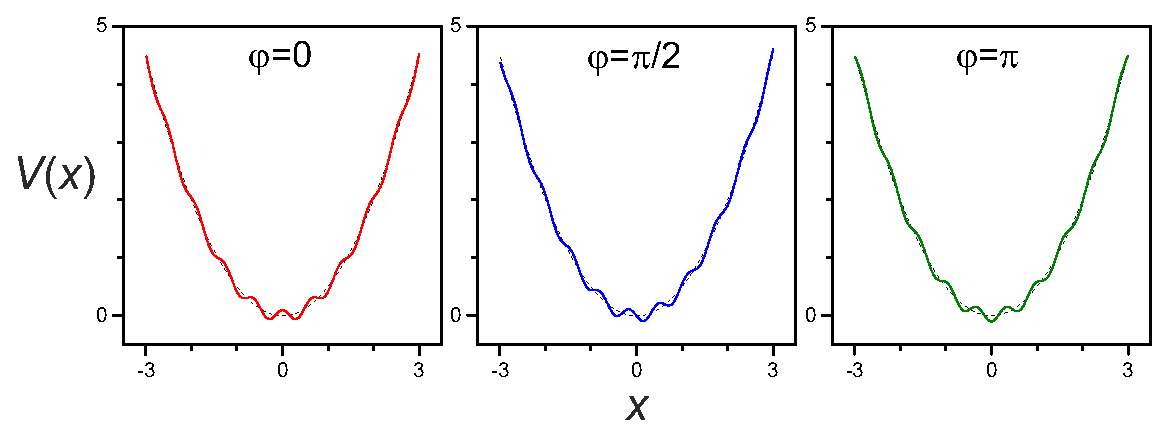
\epsfig{file=figures/porucha.eps,width=\linewidth,keepaspectratio}
			\scaption{
				Potenciál $V(x)=V_{0}(x)+V_{\mathrm{I}}(x)$ pro tři hodnoty fáze $\varphi$ (silnou barevnou čarou)
				a neporušený potenciál $V_{0}(x)$ (čárkovanou černou čarou).
				Hodnoty parametrů jsou $M=\Omega=1$, $\kappa=10$, $\lambda=0,\!1$.
				Při volbě $\hbar=0.1$ je energie neporušeného základního stavu $E_{0}^{(0)}=0,\!05$ a poruchy v jednotlivých případech
				$E_{0}^{(1)}=\left\{0,\!0082;0;-0,\!0082\right\}$.
				Střední hodnota souřadnice se posune o $0,\!082$ v případě $\varphi=\pi/2$, ve zbylých dvou případech zůstane nulová.
			}
			\label{fig:HOporucha}
		\end{figure}
	
	\item
		Oprava k vlastnímu vektoru základního stavu je podle~\eqref{eq:Perturbation1}
		\begin{equation}
			\ket{\chi_{0}^{(1)}}
				=\sum_{n=1}^{\infty}\frac{\matrixelement{n}{\cos\left(\kappa\operator{x}+\varphi\right)}{0}}{E_{0}^{(0)}-E_{n}^{(0)}}\ket{n}
				=-\frac{1}{\hbar\Omega}\sum_{n=1}^{\infty}\frac{1}{n}\Re\left[\e^{\im\varphi}\matrixelement{n}{\e^{\im\kappa\operator{x}}}{0}\right]\ket{n}\,.
		\end{equation}
		Využijeme vztahu~\eqref{eq:HOPerturbedBCH}, a maticový element v sumě vyjádříme jako
		\begin{align}
				\matrixelement{n}{\e^{\im\kappa\operator{x}}}{0}
					&=\e^{-\kappa^{2}\frac{\hbar}{4M\Omega}}\matrixelement{n}{\e^{\im\kappa\sqrt{\frac{\hbar}{2M\Omega}}\conjugate{\operator{a}}}\e^{\im\kappa\sqrt{\frac{\hbar}{2M\Omega}}\operator{a}}}{0}\nonumber\\
					&=\e^{-\kappa^{2}\frac{\hbar}{4M\Omega}}\matrixelement{n}{\e^{\im\kappa\sqrt{\frac{\hbar}{2M\Omega}}\conjugate{\operator{a}}}}{0}\nonumber\\
					&=\e^{-\kappa^{2}\frac{\hbar}{4M\Omega}}\matrixelement{n}{\sum_{k=0}^{\infty}\frac{1}{k!}\left(\im\kappa\sqrt{\frac{\hbar}{2M\Omega}}\right)^{k}\operator{a}^{\dagger k}}{0}\nonumber\\
					&=\frac{\e^{-\kappa^{2}\frac{\hbar}{4M\Omega}}}{\sqrt{n!}}\left(\im\kappa\sqrt{\frac{\hbar}{2M\Omega}}\right)^{n}\,,
			\end{align}
			takže
			\begin{align}
				\ket{\chi_{0}^{(1)}}
					&=-\frac{1}{\hbar\Omega}\sum_{n=1}^{\infty}\frac{1}{n}\frac{\e^{-\kappa^{2}\frac{\hbar}{4M\Omega}}}{\sqrt{n!}}\Re\left[\e^{\im\varphi}\left(\im\kappa\sqrt{\frac{\hbar}{2M\Omega}}\right)^{n}\right]\ket{n}\nonumber\\
					&=-\frac{1}{\hbar\Omega}\e^{-\kappa^{2}\frac{\hbar}{4M\Omega}}\sum_{n=1}^{\infty}\frac{1}{n\sqrt{n!}}\Re\left[\left(\cos{\varphi}+\im\sin{\varphi}\right)\left(\im\kappa\sqrt{\frac{\hbar}{2M\Omega}}\right)^{n}\right]\ket{n}\nonumber\\
					&=-\frac{1}{\hbar\Omega}\e^{-\kappa^{2}\frac{\hbar}{4M\Omega}}\left[
						\cos{\varphi}\sum_{n=1}^{\infty}\frac{\minus{n}}{2n\sqrt{(2n)!}}\kappa^{2n}\left(\frac{\hbar}{2M\Omega}\right)^{n}\ket{2n}\right.\nonumber\\
					&\qquad\left.-\sin{\varphi}\sqrt{\frac{\hbar}{2M\Omega}}\sum_{n=0}^{\infty}\frac{\minus{n}}{(2n+1)\sqrt{(2n+1)!}}\kappa^{2n+1}\left(\frac{\hbar}{2M\Omega}\right)^{n}\ket{2n+1}\right].
			\end{align}
			Střední hodnota operátoru souřadnice je tedy (do prvního řádu v $\lambda$)
			\begin{align}
				\matrixelement{\chi_{0}}{\operator{x}}{\chi_{0}}
					&=\sqrt{\frac{\hbar}{2M\Omega}}\left[\bra{0}+\lambda\bra{\chi_{0}^{(1)}}\right]\conjugate{\operator{a}}+\operator{a}\left[\ket{0}+\lambda\ket{\chi_{0}^{(1)}}\right]\nonumber\\
					&\approx\lambda\sqrt{\frac{\hbar}{2M\Omega}}\left[\matrixelement{0}{\operator{a}}{\chi_{0}^{(1)}}+\matrixelement{\chi_{0}^{(1)}}{\conjugate{\operator{a}}}{0}\right]\nonumber\\
					&=2\lambda\sqrt{\frac{\hbar}{2M\Omega}}\matrixelement{\chi_{0}^{(1)}}{\conjugate{\operator{a}}}{0}\nonumber\\
					&=2\lambda\sqrt{\frac{\hbar}{2M\Omega}}\frac{1}{\hbar\Omega}\e^{-\kappa^{2}\frac{\hbar}{4M\Omega}}\sin{\varphi}\sqrt{\frac{\hbar}{2M\Omega}}\,\kappa\nonumber\\
					&=\frac{\lambda\kappa}{M\Omega^{2}}\e^{-\kappa^{2}\frac{\hbar}{4M\Omega}}\sin{\varphi}
			\end{align}
			a střední hodnota kvadrátu operátoru souřadnice (opět do prvního řádu v $\lambda$)
			\begin{align}
				\matrixelement{\chi_{0}}{\operator{x}^{2}}{\chi_{0}}
					&\approx\frac{\hbar}{2M\Omega}\left[\matrixelement{0}{\operator{a}\conjugate{\operator{a}}}{0}+2\lambda\matrixelement{\chi_{0}^{(1)}}{\operator{a}^{\dagger 2}}{0}\right]\nonumber\\
					&=\frac{\hbar}{2M\Omega}\left[1+\frac{\lambda\kappa^{2}}{2M\Omega^{2}}\e^{-\kappa^{2}\frac{\hbar}{4M\Omega}}\cos{\varphi}\right]\,.
			\end{align}			

			Výsledky jsou zobrazeny na obrázku~\ref{fig:HOporucha}.
	\end{enumerate}
\end{solution}

\subsection{Van der Waalsova interakce}
\label{sec:VanDerWaals}
Uvažujte dva atomy vodíku, přičemž vektor vzájemné polohy jejich jader $\vector{R}$ míří od prvního atomu k druhému, polohy elektronů vůči příslušným atomům jsou udány vektory 
$\vector{r}_{1}$, $\vector{r}_{2}$.

Pro dostatečně velkou vzájemnou vzdálenost atomů vůči vzdálenostem jejich elektronů a při hrubé aproximaci $E_{n\geq2}^{(0)}\approx0$ (to značí, že všechny energie jednotlivých atomů vodíku kromě základních stavů berte jako nulové)
nalezněte opravu k energii základního stavu systému a rozhodněte, zda uvažovaná interakce bude přitažlivá či odpudivá.

Výpočet provádějte v adiabatické aproximaci, tj. předpokládejte, že atomy se vůči sobě nepohybují.

\begin{solution}
	Neporušený Hamiltonián je součtem Hamiltoniánů dvou neinteragujících atomů vodíku, jehož spektrum (vlastní energie a vlastní funkce) je známé.
	Oprava (porucha) pak bude dána interakcemi konstituentů jednoho atomu s konstituenty atomu druhého:
    \begin{subequations}
        \begin{align}
            \operator{H}&=\operator{H}_{0}+\operator{H}_{\ti{I}},\\
            \operator{H}_{0}&=\frac{\vectoroperator{p}_{1}^{2}}{2m}+\frac{\vectoroperator{p}_{2}^{2}}{2m}-\frac{\gamma}{\operator{r}_{1}}-\frac{\gamma}{\operator{r}_{2}},\\
            \operator{H}_{\ti{I}}&=\frac{\gamma}{\operator{R}}+\frac{\gamma}{\operator{r}}-\frac{\gamma}{\abs{\vectoroperator{R}+\vectoroperator{r}_{2}}}-\frac{\gamma}{\abs{\vectoroperator{R}-\vectoroperator{r}_{1}}}.
    	\end{align}                
    \end{subequations}
	V interakčním Hamiltoniánu souvisí jednotlivé členy postupně s interakcí kladně nabitých jader, interakcí elektronů ($\operator{r}=\abs{\vectoroperator{R}+\vectoroperator{r}_{2}-\vectoroperator{r}_{1}}$),
	interakcí prvního jádra s elektronem druhého atomu a interakcí druhého jádra s elektronem prvního atomu.

	Za předpokladu, že rozměry atomů jsou mnohem menší než jejich vzájemná vzdálenost, lze vzít jen \trick{nejnižší členy multipólového rozvoje}
	\begin{align}
		\frac{1}{\abs{\vector{R}-\vector{r}}}
		&=\frac{1}{R}-r_{i}\frac{\partial}{\partial R_{i}}\frac{1}{R}
		+\frac{1}{2}r_{i}r_{j}\frac{\partial^{2}}{\partial R_{i}\partial R_{j}}\frac{1}{R}-\dotsb=\nonumber\\
		&=\frac{1}{R}+\frac{R_{i}r_{i}}{R^{3}}
		+\frac{1}{2R^{3}}\left(3\frac{R_{i}R_{j}}{R^{2}}-\delta_{ij}\right)r_{i}r_{j}+\dotsb=\nonumber\\
		&=\frac{1}{R}+\frac{\vector{R}\cdot\vector{r}}{R^{3}}
		+\frac{1}{2R^{3}}\left(3\frac{(\vector{R}\cdot\vector{r})^{2}}{R^{2}}-r^{2}\right)+\dotsb.
	\end{align}
	Další člen multipólového rozvoje je 
	$\frac{\vector{R}\cdot\vector{r}}{2R^{5}}\left(5\frac{\left(\vector{R}\cdot\vector{r}\right)^{2}}{R^{2}}-3r^{2}\right)$.
	Jednotlivé řády multipólového rozvoje $H_{\ti{I}}$ jsou:
    \begin{subequations}
        \begin{align}
            \operator{H}_{\ti{I}}^{\hi{0}}&=0,\\
            \operator{H}_{\ti{I}}^{\hi{1}}
            &=\frac{\gamma}{\operator{R}^{3}}\left[\vectoroperator{R}\cdot\left(\vectoroperator{r}_{1}-\vectoroperator{r}_{2}\right)
            +\vectoroperator{R}\cdot\vectoroperator{r}_{2}-\vectoroperator{R}\cdot\vectoroperator{r}_{1}\right]=0,\\
            \operator{H}_{\ti{I}}^{\hi{2}}
            &=\frac{\gamma}{2\operator{R}^{3}}\left[3\frac{\left(\vectoroperator{R}\cdot\left(\vectoroperator{r}_{1}-\vectoroperator{r}_{2}\right)\right)^{2}}{\operator{R}^{2}}
            -\left(\vectoroperator{r}_{1}-\vectoroperator{r}_{2}\right)^{2}-\right.\nonumber\\
            & \qquad\left.-3\frac{\left(\vectoroperator{R}\cdot\vectoroperator{r}_{2}\right)^{2}}{\operator{R}^{2}}+\operator{r}_{2}^{2}
            -3\frac{\left(\vectoroperator{R}\cdot\vectoroperator{r}_{1}\right)^{2}}{\operator{R}^{2}}+\operator{r}_{1}^{2}\right]=\nonumber\\
            &=\frac{\gamma}{\operator{R}^{3}}\left[\vectoroperator{r}_{1}\cdot\vectoroperator{r}_{2}
            -3\frac{\left(\vectoroperator{R}\cdot\vectoroperator{r}_{1}\right)\left(\vectoroperator{R}\cdot\vectoroperator{r}_{2}\right)}{\operator{R}^{2}}\right].
        \end{align}
    \end{subequations}
	Nadále se omezíme na přiblížení $\operator{H}_{\ti{I}}\approx\operator{H}_{\ti{I}}^{(2)}$\sfootnote{
		To je vlastně interakční energie dvou dipólových momentů $\vectoroperator{d}_{1,2}=-e\,\vectoroperator{r}_{1,2}$:
		\begin{equation}
			\operator{H}_{\ti{I}}^{(2)}=\frac{1}{4\pi\epsilon_{0}}\frac{1}{R^{3}}\left[\vectoroperator{d}_{1}\cdot\vectoroperator{d}_{2}
		-3\frac{\left(\vectoroperator{R}\cdot\vectoroperator{d}_{1}\right)\left(\vectoroperator{R}\cdot\vectoroperator{d}_{2}\right)}{\operator{R}^{2}}\right].
		\end{equation}
	}.

	Ve \trick{speciálně zvolené souřadné soustavě}, ve které osa $z$ směřuje ve směru spojnice jader atomů od prvního jádra ke druhému, je
	\begin{align}
		\operator{H}_{\ti{I}}
		&=\frac{\gamma}{\operator{R}^{3}}\left[\operator{x}_{1}\operator{x}_{2}+\operator{y}_{1}\operator{y}_{2}+\operator{z}_{1}\operator{z}_{2}
		-3\frac{(\operator{R}\operator{z}_{1})(\operator{R}\operator{z}_{2})}{\operator{R}^{2}}\right]=\nonumber\\
		&=\frac{\gamma}{\operator{R}^{3}}\left[\operator{x}_{1}\operator{x}_{2}+\operator{y}_{1}\operator{y}_{2}-2\operator{z}_{1}\operator{z}_{2}\right].
	\end{align}
	přičemž $\vectoroperator{r}_{1}=(\operator{x}_{1},\operator{y}_{1},\operator{z}_{1})$ jsou složky vektoru $\vectoroperator{r}_{1}$; analogicky pro vektor $\vectoroperator{r}_{2}$.

	Neporušený základní stav dvou volných atomů vodíku je dán vlnovou funkcí
	\begin{equation}
	\ket{\phi_{1}}=\ket{n=1\,l=0\,m=0}_{1}\ket{n=1\,l=0\,m=0}_{2}\equiv\ket{1}\ket{2}
	\end{equation}
	(při použití zjednodušeného označení $\ket{1,2}\equiv\ket{n=1\,l=0\,m=0}_{1,2}$).
	Atomy jsou nerozlišitelné, vlnový vektor tudíž musí být symetrický nebo antisymetrický vůči záměně částic.\sfootnote{Pro úplnou analýzu je potřeba zahrnout i spinový stav elektronů; pro účely této úlohy stačí uvažovat, že spin elektronů se složí na antisymetrický singletní stav, aby celková vlnová funkce byla antisymetrická.}
	To je splněno.

	\emph{1. oprava k energii} je dle poruchové teorie
	\begin{align}
		E_{11}^{\hi{1}}&=\matrixelement{\phi_{1}}{\operator{H}_{\ti{I}}}{\phi_{1}}=\nonumber\\
		&=\frac{\gamma}{\operator{R}^{3}}\Big[\matrixelement{1}{\operator{x}_{1}}{1}\matrixelement{2}{\operator{x}_{2}}{2}+\matrixelement{1}{\operator{y}_{1}}{1}\matrixelement{2}{\operator{y}_{2}}{2}
		-2\matrixelement{1}{\operator{z}_{1}}{1}\matrixelement{2}{\operator{z}_{2}}{2}\Big].
	\end{align}
	K určení maticových elementů lze využít výběrová pravidla podle Wigner-Eckartova teorému~\eqref{eq:WignerEckartSelectionRules}.
	Komponenty vektorových operátorů $\vectoroperator{r}_{1,2}$ se vyjádří pomocí komponent tenzorových operátorů 1. řádu, viz~\eqref{eq:VectorTensor}). Je tedy $\lambda=1$ a jednotlivé komponenty jsou odlišeny indexem $\mu$.
	Výběrová pravidla pak dávají $J=j\pm1$ a $M=m+\mu$, kde v našem případě $J\equiv l=0$, $j\equiv l=0$, $M=m=0$.
	To není splněno pro žádnou ze složek operátorů $\vectoroperator{r}_{1,2}$, takže všechny maticové elementy na pravé straně výrazu pro 1. opravu jsou nulové.\sfootnote{
		To úzce souvisí s tím, že dipólový moment atomů v základním stavu je nulový.
	}

	\emph{2. oprava k energii} základního stavu dává
	\begin{align}
        E_{11}^{\hi{2}}
            &=\sum_{\substack{n_{1}\neq1 \\ n_{2}\neq1 \\ l_{1}\,m_{1}\,l_{2}\,m_{2}}}
                \frac{\abs{\bra{2}\bra{1}\operator{H}_{\ti{I}}\ket{n_{1}\,l_{1}\,m_{1}}\ket{n_{2}\,l_{2}\,m_{2}}}^{2}}
                {2E_{1}^{\hi{0}}-E_{n_{1}}^{\hi{0}}-E_{n_{2}}^{\hi{0}}}\approx\nonumber\\
            &\approx\frac{1}{2E_{1}^{\hi{0}}}\sum\bra{2}\bra{1}\operator{H}_{\ti{I}}\ket{n_{1}\,l_{1}\,m_{1}}\ket{n_{2}\,l_{2}\,m_{2}}
                \bra{n_{1}\,l_{1}\,m_{1}}\bra{n_{2}\,l_{2}\,m_{2}}\operator{H}_{\ti{I}}\ket{1}\ket{2}=\nonumber\\
            &=\frac{1}{2E_{1}^{\hi{0}}}\bra{2}\bra{1}\operator{H}_{\ti{I}}\left(\operator{1}-
                \ket{1}\ket{2}\bra{2}\bra{1}\right)\operator{H}_{\ti{I}}\ket{1}\ket{2}=\nonumber\\
            &=\frac{1}{2E_{1}^{\hi{0}}}\bra{2}\bra{1}\operator{H}_{\ti{I}}^{2}\ket{1}\ket{2},
	\end{align}
	kde se provedla \trick{hrubá aproximace $E_{n\geq2}^{\hi{0}}\approx0$}, využily se relace úplnosti a znalost nulovosti maticových elementů $\bra{2}\bra{1}\operator{H}_{\ti{I}}\ket{1}\ket{2}$.
	Při formálně zcela správném řešení je nutné uvažovat nerozlišitelnost částit, avšak výsledek bude stejný (díky užití relací úplnosti).

	Kvadrát Hamiltoniánu poruchy je
	\begin{equation}
		\operator{H}_{\ti{I}}^{2}=\frac{\gamma^{2}}{\operator{R}^{6}}\left[\operator{x}_{1}^{2}\operator{x}_{2}^{2}+\operator{y}_{1}^{2}\operator{y}_{2}^{2}+4\operator{z}_{1}^{2}\operator{z}_{2}^{2}
			+2\operator{x}_{1}\operator{x}_{2}\operator{y}_{1}\operator{y}_{2}-4\operator{x}_{1}\operator{x}_{2}\operator{z}_{1}\operator{z}_{2}-4\operator{y}_{1}\operator{y}_{2}\operator{z}_{1}\operator{z}_{2}\right].
	\end{equation}
	Maticový element pro smíšené členy (poslední tři členy v závorce) se vynuluje díky symetrii základního stavu.\sfootnote{
		Toto lze opět dokázat pomocí Wigner-Eckartova teorému.
		Na základě příkladu~\ref{sec:DyadicProduct} lze dyadický součin dvou vektorových operátorů $\vectoroperator{R}$, $\vectoroperator{S}$ vyjádřit pomocí tenzorových operátorů nultého, prvního a druhého řádu.
		Speciálně pro $\vectoroperator{R}=\vectoroperator{S}$ a pro smíšené složky $R_{j}$, $R_{k}$, $j\neq k$ platí
		\begin{align}
			\operator{R}_{1}\operator{R}_{2}&=\frac{\tensoroperatorcomponent{T}{2}{2}-\tensoroperatorcomponent{T}{2}{-2}}{2\im},
			&\operator{R}_{2}\operator{R}_{3}&=-\frac{\tensoroperatorcomponent{T}{2}{1}+\tensoroperatorcomponent{T}{2}{-1}}{2\im},
			&\operator{R}_{1}\operator{R}_{3}&=-\frac{\tensoroperatorcomponent{T}{2}{1}-\tensoroperatorcomponent{T}{2}{-1}}{2},
		\end{align}
		dají se tedy vyjádřit pomocí tenzorového operátoru řádu $\lambda=2$ s projekcí $\mu\neq0$.
		Po nahrazení $(\operator{R}_{1},\operator{R}_{2},\operator{R}_{3})=(\operator{x}_{1,2},\operator{y}_{1,2},\operator{z}_{1,2})$ se dospějena základě výběrových pravidel Wigner-Eckartova teorému k závěru, že libovolný maticový element $\matrixelement{100}{R_{j}R_{k}}{100}=0$, $j\neq k$.
	}
	Ze symetrie také vyplývá
	\begin{equation}
		\matrixelement{1}{\operator{x}_{1}^{2}}{1}=\matrixelement{1}{\operator{y}_{1}^{2}}{1}=\matrixelement{1}{\operator{z}_{1}^{2}}{1}=\frac{1}{3}\matrixelement{1}{\operator{r}_{1}^{2}}{1},
	\end{equation}
	takže druhou opravu k energii lze nakonec vyjádřit jako
	\begin{align}
		E_{11}^{\hi{2}}
			&=\frac{\gamma^{2}}{2E_{1}^{\hi{0}}R^{6}}\left[
				\matrixelement{1}{\operator{x}_{1}^{2}}{1}\matrixelement{2}{\operator{x}_{2}^{2}}{2}+
				\matrixelement{1}{\operator{y}_{1}^{2}}{1}\matrixelement{2}{\operator{y}_{2}^{2}}{2}+
				4\matrixelement{1}{\operator{z}_{1}^{2}}{1}\matrixelement{2}{\operator{z}_{2}^{2}}{2}
				\right]=\nonumber\\
			&=\frac{\gamma^{2}}{2E_{1}^{\hi{0}}R^{6}}\,\frac{6}{9}\matrixelement{1}{\operator{r}_{1}^{2}}{1}\matrixelement{2}{\operator{r}_{2}^{2}}{2}
            \label{eq:VanDerWaalsPerturbation2}
	\end{align}

	Zbytek úlohy se dořeší v $x$-reprezentaci.
	Energetické hladiny atomu vodíku jsou
	\begin{equation}
		E_{n}^{\hi{0}}=-\frac{\gamma}{2a_{0}}\frac{1}{n^{2}}
	\end{equation}
	a radiální část vlnové funkce základního stavu zní\sfootnote{
		Celá vlnová funkce základního stavu je $\braket{r,\theta,\phi}{100}=R_{10}(r)Y_{00}(\theta,\phi)$, 
		kde $Y_{00}(\theta,\phi)=1/\sqrt{4\pi}$. 
		Úhlovou a radiální část lze od sebe odseparovat a zde se počítá maticový element operátoru, který na úhlovou část nepůsobí, proto stačí uvažovat pouze radiální část.
	}
	\begin{equation}
		\label{eq:HydrogenR10}
		R_{10}(r)=\braket{r}{100}=\frac{2}{a_{0}^{\frac{3}{2}}}\e^{-\frac{r}{a_{0}}},
	\end{equation}
	kde $a_{0}=\hbar^{2}/\gamma m$ je Bohrův poloměr.
	Maticový element je dán integrálem
	\begin{align}
		\matrixelement{100}{\operator{r}^{2}}{100}
		&=\frac{4}{a_{0}^{3}}\int_{0}^{\infty}\e^{-\frac{r}{a_{0}}}\,r^{2}\e^{-\frac{r}{a_{0}}}\,r^{2}\d r=\nonumber\\
		&=\frac{4}{a_{0}^{3}}\int_{0}^{\infty}r^{4}\e^{-\frac{2r}{a_{0}}}\d r=\nonumber\\
		&=-\frac{4}{a_{0}^{3}}\,4\frac{a_{0}}{2}\int_{0}^{\infty}r^{3}\e^{-\frac{2r}{a_{0}}}\d r=\dotsb=\nonumber\\
		&=-\frac{4}{a_{0}^{3}}\,4!\left(\frac{a_{0}}{2}\right)^{5}\left[\e^{-\frac{2r}{a_{0}}}\right]_{0}^{\infty}=\nonumber\\
		&=\frac{4}{a_{0}^{3}}\,24\left(\frac{a_{0}}{2}\right)^{5}=\nonumber\\
		&=3a_{0}^{2},
	\end{align}
	který po dosazení do vztahu pro 2. opravu energie~\eqref{eq:VanDerWaalsPerturbation2} dá konečný výsledek
	\begin{equation}
		E_{11}^{\hi{2}}=\frac{3\gamma^{2}a_{0}^{4}}{E_{1}^{\hi{0}}R^{6}}=-\frac{6\gamma a_{0}^{5}}{R^{6}}.
	\end{equation}

	Oprava je záporná, lze z ní tedy usuzovat na přitažlivost sil mezi atomy a na její rychlý pokles s narůstající vzdáleností.

	Atomy nemusí být nutně vodíkové, výsledek platí i pro jiné atomy nebo molekuly,
	pouze musí dostatečně přesně platit, že na tento systém lze nahlížet jako na soustavu kladně nabitého centra 
	(jádro + elektrony z vnitřních slupek) a okolo obíhající valenční elektron.
	Pak vidíme, že Van der Waalsova síla je tím větší, čím jsou větší rozměry atomů.

	Zatímco pro základní stav je 1. oprava poruchové teorie k nulová, pro excitované stavy již tomu tak být nemusí.
	To znamená, že atomy v excitovaných stavech se budou ovlivňovat silněji na velkých vzdálenostech, velikost opravy bude klesat jen jako $\sim1/R^{3}$.
	Navíc excitované stavy mohou být degenerované a je nutné použít degenerovanou poruchovou teorii.

	Ačkoliv jsou jednotlivé dipólové momenty atomů v základním stavu nulové (dipólový moment $\equiv$ střední hodnota operátoru dipólového momentu),
	jsou Van der Waalsovy síly projevem dipól-dipólové interakce.
	Je to důsledek toho, že záladní stav není vlastním stavem dipólového operátoru $\vectoroperator{d}$.
		
	Detaily ohledně Van der Waalsovy síly naleznete v přehledovém článku~\cite{Margenau1939} či v učebnici~\cite{Formanek2004}, kapitola 10.10.3.
\end{solution}
